\section{Two-flavor quark-meson model}

\TODO{move this to the start?
The linear sigma model is an effective low-energy model of quantum chromodynamics, so accordingly we should take it seriously only in terms of the shifted fields around the stable ground states, and not in terms of the unshifted fields around the unstable equilibrium at the top of the Mexican hat.
}

\TODO{two inconsistencies: (1) match couplings at tree level although using one-loop potential. (2) neglecting bosonic one-loop contribution to effective potential (this is consistent in $N_c\rightarrow \infty$ limit, but inconsistent in terms of number of loops)}

\begin{figure}
\centering
\tikzsetnextfilename{potential}
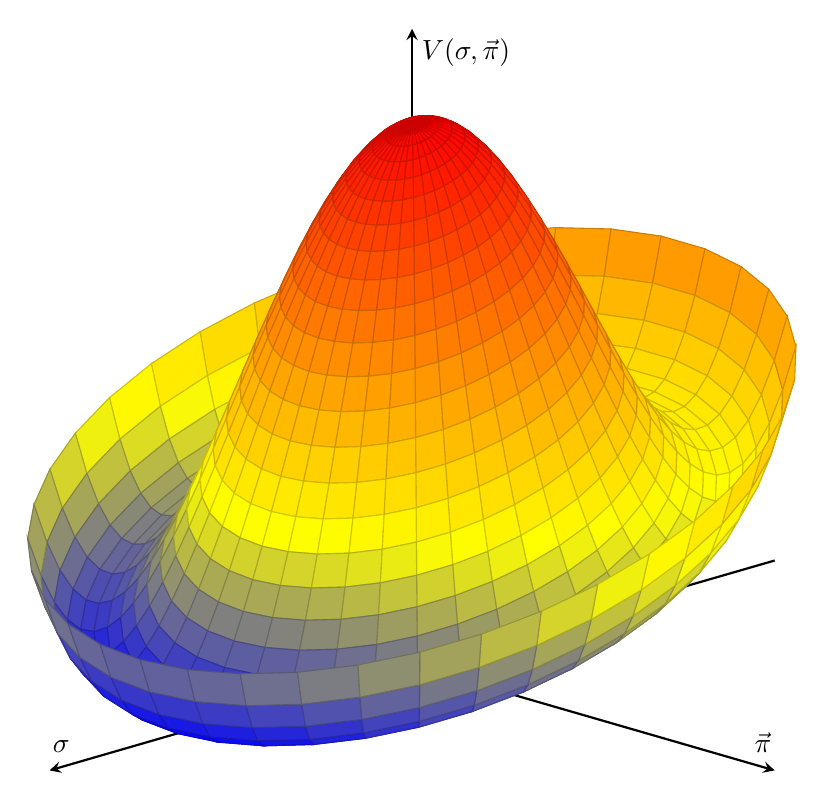
\begin{tikzpicture}
\begin{axis}[
	width = 20cm, height=15cm,
	%title = {Potential},
	xlabel = $\sigma$, ylabel = $\vec\pi$, zlabel = {$V(\sigma,\vec\pi)$},
	xmin=-4.0, xmax=+4.0, ymin=-4.0, ymax=+4.0, zmin=0, zmax=2.2,
	xtick=\empty, ytick=\empty, ztick=\empty,
	axis lines=center,
	axis line style = thick,
	view={135}{25},
	%colormap/blackwhite, mesh/interior colormap name=plasmarev,
]
	\addplot3 [surf, thin, domain=0:3.0, domain y=0:2*pi, samples=30, samples y=40, z buffer=sort] ({x*cos(deg(y))},{x*sin(deg(y))},{-1/2*((x*cos(deg(y)))^2+(x*sin(deg(y)))^2) + 1/24*((x*cos(deg(y)))^2+(x*sin(deg(y)))^2)^2 + 3/2 - 0.15*x*cos(deg(y)) + 0.15*sqrt(6)});
	%\addplot3 [domain=0:2*pi, samples=50, samples y=1] ({sqrt(6)*cos(deg(x))},{sqrt(6)*sin(deg(x))},{0});
\end{axis}
\end{tikzpicture}
\caption{\label{fig:lsm:potential}%
	A two-dimensional realization of the potential \eqref{eq:lsm:potential} looks like a Mexican hat, tilted along the $\sigma$-axis by the explicit symmetry breaking parameter $h$.
	If $h = 0$, the hat is upright with a continuous range of minima around $\sigma^2 + \vec\pi^2 = -6m^2 / \lambda$;
	while if $h \neq 0$, the hat is tilted and has the discrete minimum \eqref{eq:lsm:ground_state_implicit}.
}
\end{figure}

\TODO{justify this effective MODEL from QCD. Expand QCD $\lagr$ at low energy?}

\TODO{rewrite presentation!}

The Lagrangian density for the linear sigma model coupled to quarks is
\begin{equation}
	\lagr = \sum_{c=1}^{N_c} \bar{q}_c \Big[ i \slashed\partial + \mu \gamma^0 - g \big( \sigma + i \gamma^5 \vec\tau \cdot \vec\pi \big) \Big] q_c
	      + \frac12 \Big[ \big( \partial_\mu \sigma \big)^2 + \big( \partial_\mu \vec\pi \big)^2 \Big] - \pot(\sigma,\vec\pi) ,
\label{eq:lsm:lagrangian}
\end{equation}
with the meson potential
\begin{equation}
	\pot(\sigma, \vec\pi) = \frac{m^2}{2} \big( \sigma^2 + \vec\pi^2 \big) + \frac{\lambda}{4!} \big( \sigma^2 + \vec\pi^2 \big)^2 - h \sigma .
\label{eq:lsm:potential}
\end{equation}
Here $q_c = [u_c, d_c]^T$ represents quarks of the $N_c = 3$ colors red, green and blue and the $N_f = 2$ flavors up and down, so $(q_c)_f$ make up a total of $N_c \times N_f = 6$ Dirac spinors.
In addition, $\sigma$ and $\vec\pi = [\pi^+, \pi^-, \pi^0]^T$ are four bosonic scalar fields representing sigma and pion mesons.
At this point, the quarks are massless Dirac fermions whose conserved charge densities $j^0 = \bar\psi \gamma^0 \psi$ are coupled to quark chemical potentials $\mu = \diag(\mu_u, \mu_d)$, interacting with a Yukawa coupling of strength $g$ that models the strong force \TODO{non-mentioned comment in Møte 4}, where $\vec\tau$ are the Pauli matrices \eqref{eq:tft:pauli_matrices}.
\TODO{$SU(2)_L$, $SU(2)_R$, etc.?}

We will study quantum fluctuations to first nonzero order around the classical ground state.
The classical ground state is given by a pair of constant meson fields $\sigma = \avg{\sigma}$ and $\pi = \avg{\pi}$ that minimizes the meson potential \TODO{IN VACCUUM, SEE (10) IN \cite{ref:lsm_2f}, this asserts that $\avg{\bar{q}q}=0$ in vacuum?}.
The dependence on the three fields $\vec{\pi}$ is spherically symmetric, so if we imagine collapsing this three-dimensional field down to one dimension, the potential looks like the Mexican hat drawn in \cref{fig:lsm:potential}, tilted by the symmetry breaking parameter $h$.
Provided that $h \neq 0$, the minimum of the classical ground state is discrete and located at 
%Let us warm up with the special case $h = 0$, where the potential is symmetric under rotation of $[\sigma, \vec{\pi}]^T$ in $O(4)$ and looks like an upright Mexican hat with a continuous curve of minima along $\sigma^2 + \vec{\pi}^2 = -6m^2/\lambda$.
%Committing to one of these classical ground states, such as $\sigma=\avg{\sigma}=\sqrt{-6m^2/\lambda}$ and $\vec{\pi}=\avg{\vec{\pi}}=\vec{0}$,
%and shifting the fields to $\sigma \rightarrow \avg{\sigma} + \tilde{\sigma}$ and $\vec{\pi} \rightarrow \avg{\vec{\pi}} + \tilde{\vec{\pi}}$ then spontaneously breaks the symmetry to rotations of the pion quantum fluctuations $\tilde{\vec{\pi}}$ in $O(3)$ only,
%giving rise to three massless Goldstone bosons that we interpret as pions.
%We will work in the general case, however, where $h \neq 0$ tilts the hat so that it has a global minimum at $\sigma=\avg{\sigma}$ and $\vec{\pi}=\avg{\vec{\pi}}$ determined by
\begin{equation}
	\vec{\pi} = \avg{\vec{\pi}} = \vec{0}
	\quad \text{and} \quad
	\sigma = \avg{\sigma}
	\quad \text{where} \quad
	%\pdv{\pot}{\sigma}_{(\sigma,\vec\pi)=(\avg{\sigma},\vec{0})} = m^2 \avg{\sigma} + \frac{\lambda}{6} \avg{\sigma}^3 - h = 0.
	\pdv{\pot}{\sigma} = m^2 \avg{\sigma} + \frac{\lambda}{6} \avg{\sigma}^3 - h = 0.
\label{eq:lsm:ground_state_implicit}
\end{equation}
%We assume that $h \neq 0$, but will briefly discuss the qualitatively different behavior in the special case $h = 0$ in a moment.
To account for quantum fluctuations $\tilde{\sigma}$ and $\tilde{\vec{\pi}}$ around the classical ground state \eqref{eq:lsm:ground_state_implicit}, we shift
\begin{equation}
	\sigma \rightarrow \avg{\sigma} + \tilde{\sigma}
	\qquad \text{and} \qquad
	\vec\pi \rightarrow \avg{\vec\pi} + \tilde{\vec\pi}.
\label{eq:lsm:field_shift}
\end{equation}
Up to first nonzero order in the quantum fluctuations $\tilde\sigma$ and $\tilde{\vec\pi}$, the Lagrangian \eqref{eq:lsm:lagrangian} is now
\begin{equation}
	\lagr = \sum_{c=1}^{N_c} \bar{q}_c \Big[ i \slashed\partial + \mu \gamma^0 - m_q \Big] q_c
	      + \frac12 \left[ \left( \partial_\mu \tilde{\sigma} \right)^2 + \left( \partial_\mu \tilde{\vec\pi} \right)^2 \right] - \pot , %\pot(\avg{\sigma}+\tilde{\sigma},\avg{\vec\pi}+\tilde{\vec\pi}) ,
\end{equation}
where the quark fields $q$ have acquired field-dependent effective masses
\begin{equation}
	m_q(\avg{\sigma}) = g \avg{\sigma} .
\label{eq:lsm:mass_quark}
\end{equation}
The potential \eqref{eq:lsm:potential} up to second order in the shifted fields is
\TODO{no, I have not included $h \tilde{\sigma}$!}
\begin{equation}
	\pot \taylor \frac12 m^2 \avg{\sigma}^2 + \frac{\lambda}{4!} \avg{\sigma}^4 - h \avg{\sigma} + \frac12 m_\sigma^2 \sigma^2  + \frac12 m_\pi^2 \vec\pi^2 ,
	%V(\sigma, \vec\pi) \taylor -\frac12 m^2 \avg{\sigma}^2 + \frac{\lambda}{4!} \avg{\sigma}^4 + \frac12 (\sqrt{2} m)^2 \sigma^2 .
	%V(\sigma, \vec\pi) \taylor -\frac{3 m^4}{2 \lambda} + \frac12 (\sqrt{2} m)^2 \sigma^2 .
\label{eq:lsm:potential_shifted}
\end{equation}
where the $\sigma$ and $\vec\pi$ fields have acquired the effective masses
\begin{subequations}
\begin{align}
	m_\sigma^2 &= \pdv[2]{\pot}{\sigma}_{\substack{\sigma=\avg{\sigma}\\\vec{\pi}=\avg{\vec{\pi}}}}    = m^2 + \frac{\lambda}{2} \avg{\sigma}^2 \equalexplabove{\text{by \eqref{eq:lsm:ground_state_implicit}}} \frac{3h}{\avg{\sigma}} - 2 m^2 , \label{eq:lsm:mass_sigma} \\
	m_\pi^2    &= \pdv[2]{\pot}{\vec{\pi}}_{\substack{\sigma=\avg{\sigma}\\\vec{\pi}=\avg{\vec{\pi}}}} = m^2 + \frac{\lambda}{6} \avg{\sigma}^2 \equalexplbelow{\text{by \eqref{eq:lsm:ground_state_implicit}}} \frac{h}{\avg{\sigma}} , \label{eq:lsm:mass_pi}
\end{align}%
\label{eq:lsm:mass_sigmapi}%
\end{subequations}%
The fate of the pion mass \eqref{eq:lsm:mass_pi} is determined by the presence of the symmetry breaking parameter $h$.
In the special case $h = 0$, the potential \eqref{eq:lsm:potential} shown in \cref{fig:lsm:potential} is rather shaped like an upright Mexican hat and is symmetric under rotations of $[\sigma,\vec{\pi}]^T$ in $O(4)$.
It then no longer has the \emph{discrete} minimum \eqref{eq:lsm:ground_state_implicit}, but a \emph{continuous} range of minima along the ``brim'' $\sigma^2 + \vec{\pi}^2 = -6m^2/\lambda$ of the hat.
Upon committing to one of these classical ground states, such as $\sigma=\avg{\sigma}=\sqrt{-6m^2/\lambda}$ and $\vec{\pi}=\avg{\vec{\pi}}=\vec{0}$ and performing the field shift \eqref{eq:lsm:field_shift},
the symmetry is \emph{spontaneously} broken down to rotations of only the pion quantum fluctuations $\tilde{\vec{\pi}}$ in $O(3)$.
This gives rise to three Goldstone bosons that we interpret as \emph{massless} pions, as confirmed by equation \eqref{eq:lsm:mass_pi} with $h = 0$.
We work in the general case, however, where $h \neq 0$ instead breaks the symmetry \emph{explicitly} by tilting the hat so it has the discrete minimum \eqref{eq:lsm:ground_state_implicit}, ultimately producing \emph{massive} pions, like those observed in nature.

\begin{table}
\centering
\begin{tabular}{ l r }
	\toprule
	Parameter   & Value                                 \\
	\midrule
	$g$         & $\SI{3.23}{}$                         \\
	$\lambda$   & $-\SI{215.4}{}$                        \\
	$m^2$       & $-(\SI{539.8}{\mega\electronvolt})^2$ \\
	$h$         & $(\SI{121.0}{\mega\electronvolt})^3$  \\
	\bottomrule
\end{tabular}
\hfill
\begin{tabular}{ l r r }
	\toprule
	Physical variable & Model value                             & Experimental value                      \\
	\midrule
	$f_\pi$           & $\textbf{\SI{93}{\mega\electronvolt}}$  & \TODO{?}                                         \\
	\midrule
	$m_u=m_d$         & $\textbf{\SI{300}{\mega\electronvolt}}$ & \TODO{?}                                         \\
	\midrule
	$m_\sigma$        & $\textbf{\SI{800}{\mega\electronvolt}}$ & \SI{400}{}-\SI{700}{\mega\electronvolt}          \\
	$m_\pi$           & $\textbf{\SI{138}{\mega\electronvolt}}$ & \SI{138}{\mega\electronvolt}                     \\
	\bottomrule
\end{tabular}
\caption{\label{tab:lsm2f:parameters}%
Parameter fit for the two-flavor linear sigma model in vacuum compared to experimental values from \cite{ref:pdg_review_2021}.
The \textbf{bold values} in the right table are used as input to determine the four model parameters in the left table.
\TODO{value of $m_\sigma$?}
}
\end{table}

We determine the four parameters $g$, $h$, $m$ and $\lambda$ in the original Lagrangian \eqref{eq:lsm:lagrangian} from values of $m_q$, $m_\pi$, $m_\sigma$ and $\avg{\sigma}$ in vacuum.
Inverting equations \eqref{eq:lsm:ground_state_implicit}, \eqref{eq:lsm:mass_sigmapi} and \eqref{eq:lsm:mass_quark}, we then find the parameters
\begin{equation}
	g       = \frac{m_q}{f_\pi}, \quad % &\qquad& \text{(by \eqref{eq:lsm:mass_quark})} , \\
	h       = m_\pi^2 f_\pi, \quad % &\qquad& \text{(by \eqref{eq:lsm:mass_pi})} , \\
	m^2     = \frac{3m_\pi^2 - m_\sigma^2}{2} \quad \text{and} \quad % &\qquad& \text{(by \eqref{eq:lsm:mass_sigma})} , \\
	\lambda = \frac{3 m_\sigma^2 - 3 m_\pi^2}{f_\pi^2} .    % &\qquad& \text{(by \eqref{eq:lsm:ground_state_implicit})} .
\label{eq:lsm:parameters}
\end{equation}
The input values and output parameters are shown in \cref{tab:lsm2f:parameters}.

According to what we learned in \cref{chap:tft} in \cref{eq:tft:boson_partition_function_momentum_out} and \eqref{eq:tft:dirac_partition_function_first},
the exact partition function corresponding to this theory is obtained by a path integral over periodic bosonic fields and anti-periodic fermionic fields, weighted by a Euclidean action in imaginary time:
\TODO{sign in exponent?}
\begin{equation}
	Z = \oint_- \pathintdif \bar{q} \oint_- \pathintdif q \oint_+ \pathintdif \sigma \oint_+ \pathintdif \vec\pi \exp \left\{ \int_0^\beta \dif \tau \int_V \dif^3 x \, \lagr_E[\bar{q}, q, \sigma, \vec\pi]  \right\} .
\end{equation}
As before, we are interested in $\log Z$ so we can calculate the thermodynamic quantities \eqref{eq:tft:average_quantities} and ultimately an equation of state $\epsilon(P)$, so we can solve the Tolman-Oppenheimer-Volkoff equation \eqref{eq:tov:tovsys}.
Here we will account for quantum effects of the quarks by treating them up to quadratic order (or one-loop),
but calculate only to zeroth order (or tree-level) in the meson fields and hence consider them only at the classical level.
\TODO{a priori include bosonic fluctuations, but then they vanish in the $T=0$ limit due to \eqref{eq:tft:real_scalar_field_partition_function}}
The partition function then reads
\begin{equation}
\begin{split}
	Z &\taylor \oint_- \pathintdif \bar{q} \oint_- \pathintdif q \\
	  &\times  \exp \left\{ \int_0^{\beta} \dif \tau \int_V \dif^3 x \left[ \sum_{c=1}^{N_c} \bar{q}_c \left( i \slashed\partial -m_q + \mu \gamma^0 \right) q_c - \frac12 m^2 \avg{\sigma}^2 - \frac{\lambda}{4!} \avg{\sigma}^4 + h \avg{\sigma} \right] \right\} \\
	  &=       \prod_{f=1}^{\smash{N_f}} \prod_{c=1}^{\smash{N_c}} \oint_- \pathintdif \bar{q}_f^c \oint_- \pathintdif q_f^c \\
	  &\times  \exp \left\{ \int_0^{\beta} \dif \tau \int_V \dif^3 x \left[ \sum_{f=1}^{\smash{N_f}} \sum_{c=1}^{N_c} \bar{q}_f^c \left( i \slashed\partial - m_q + \mu_f \gamma^0 \right) q_f^c - \frac12 m^2 \avg{\sigma}^2 - \frac{\lambda}{4!} \avg{\sigma}^4 + h \avg{\sigma} \right] \right\}.
\end{split}
\end{equation}
The two last terms in the exponential are independent of the fields, so
\begin{equation}
\begin{split}
	\log Z &= -\frac12 \beta V m^2 \avg{\sigma}^2 - \frac{\lambda}{4!} \beta V \avg{\sigma}^4 + \beta V h \avg{\sigma} \\
	       &+ \sum_{f=1}^{N_f} \sum_{c=1}^{N_c} \log \oint_- \pathintdif \bar{q}_f^c \oint_- \pathintdif q_f^c \exp \left\{ \int_0^\beta \dif \tau \int_V \dif^3 x \, \bar{q}_f^c (i \slashed\partial + \mu_f \gamma^0 - m_q) q_f^c \right\} .
\end{split}
\end{equation}
We have already spent a great deal of effort in calculating the path integral in the last term,
starting from \cref{eq:tft:dirac_partition_function_first} and resulting in the expression \eqref{eq:tft:dirac_partition_function}.
Here, we get an additional factor $\sum_{c=1}^{N_c} = N_c$ from the color sum because the summand is independent of $c$,
while the flavor sum $\sum_{f=1}^{\smash{N_f}}$ yields $N_f$ terms that differ only by the unique chemical potentials $\mu_f$ associated with each quark flavor. 
Thus, we obtain
\begin{equation}
\begin{split}
	\log Z &= -\frac12 \beta V m^2 \avg{\sigma}^2 - \frac{\lambda}{4!} \beta V \avg{\sigma}^4 + \beta V h \avg{\sigma} \\
	       &+ 2 V N_c \sum_{f=1}^{N_f} \int \frac{\dif^3 p}{(2 \pi)^3} \left\{ \beta E(\vec{p}) + \log \left[ e^{-\beta (E(\vec{p}) - \mu_f)}+1 \right] + \log \left[ e^{-\beta (E(\vec{p}) + \mu_f)} + 1\right] \right\} ,
\end{split}
\label{eq:lsm:potential_divergent_logz0}
\end{equation}
where the dispersion relation is
\begin{equation}
	E(\vec{p}) = \sqrt{p^2 + m_q^2} .
\end{equation}
We can assess our approximation of treating bosons to tree-level, but fermions to loop-level from expression \eqref{eq:lsm:potential_divergent_logz0}.
The fermionic contribution in the second line is of order $\bigo(N_c^1)$, while the bosonic contribution in the first line is only of order $\bigo(N_c^0)$.
Thus, this approximation is exact in the so-called large-$N_c$ limit $N_c \gg 1$.
The million-dollar question that decides the accuracy of the approximation is then whether $N_c = 3 \gg 1$.
Although it may sound like we are not making a great case for ourselves, this is the most common treatment in the literature, and thus the strategy that we will adopt for now.
However, we will later return to this issue and consistently treat both bosons and fermions to the one-loop level, building upon the results of \cite{ref:jo_lsm_renormalization}.
\TODO{will I return to this later? RPA -- one-loop bosons too!}

Like in \cref{chap:nstars}, we assume that the chemical potentials are chosen so that anti-particles are more or less absent, so we drop their contribution in the last term in the second line.
From the middle term in the second line, we obtained the contribution $\log Z = \beta V P$ with the pressure \eqref{eq:nstars:pressure_zeroT} in the zero-temperature approximation, which we will continue to use.
This time, however, we will renormalize the infinite vacuum contribution from the first term in the second line, instead of simply dropping it, like we did back in \cref{chap:nstars}.
Thus, we obtain
\begin{equation}
\begin{split}
	\log Z &= -\frac12 \beta V m^2 \avg{\sigma}^2 - \frac{\lambda}{4!} \beta V \avg{\sigma}^4 + \beta V h \avg{\sigma} + N_c N_f \log Z_0 \\
	       &+ N_c \frac{m_q^4 \beta V}{24 \pi^2} \sum_{f=1}^{N_f} \left[ (2 x_f^3 - 3x_f) \sqrt{x_f^2 + 1} + 3 \asinh x_f \right],
\end{split}
\end{equation}
where $x_f = p_f / m_q$ are normalized Fermi momenta, $\mu_f = \smash{\sqrt{p_f^2 + m_q^2}}$ are Fermi energies and the vacuum contribution is
\begin{equation}
	\log Z_0 = 2 \beta V \int \frac{\dif^3 p}{(2 \pi)^3} \sqrt{p^2 + m_q^2 } .
\label{eq:lsm:vacuum_contribution_3dim}
\end{equation}
To renormalize the vacuum contribution, let us use dimensional regularization in the minimal subtraction scheme.
In $d = 3 - 2 \epsilon$ spatial dimensions, the vacuum contribution is
\begin{equation}
\begin{split}
	\log Z_0 &= 2 \beta V \Lambda^{3-d} \int \frac{\dif^d p}{(2 \pi)^d} \sqrt{p^2 + m_q^2} \\
	         &= 2 \beta V \Lambda^{3-d} \frac{2 \pi^{d/2}}{\Gamma(d/2)} \int_0^\infty \frac{\dif p \, p^{d-1}}{(2 \pi)^d} \sqrt{p^2 + m_q^2} .
\end{split}
\label{eq:lsm:vacuum_contribution_ddim}
\end{equation}
%\TODO{what happens to the dimensions of the potential $V$ (as consequence of requiring $\log Z$ to be dimensionless)? $V \rightarrow V \lambda^{-2\epsilon}$?}
We have also multiplied the integral by $\Lambda^{3-d}$,
where $\Lambda$ is some number with $\unit{\Lambda} = \unit{p}$,
so that $\unit{\lambda^{3-d} \dif^d p} = \unit{\dif^3 p}$ and $\log Z$ remains dimensionless in all dimensions.
There is nothing that forbids us from doing so, 
as the regulator still does its only job of reducing the new integral \eqref{eq:lsm:vacuum_contribution_ddim} to the old integral \eqref{eq:lsm:vacuum_contribution_3dim} when we send $\epsilon \rightarrow 0$,
only now in a way that is well-defined in all dimensions.
The momentum integral can be written as an analytical continuation of the \emph{Beta function} \cite{ref:beta_function}
\begin{equation}
	B(x,y) = \int_0^\infty \dif t \, \frac{t^{x-1}}{(1+t)^{x+y}} = \frac{\Gamma(x) \Gamma(y)}{\Gamma(x+y)}
\end{equation}
if we substitute $t = p^2/m_q^2$ with $\dif t = 2 p \dif p / m_q^2$.
We then find
\begin{equation}
\begin{split}
	\log Z_0 &= \beta V \Lambda^{3-d} m_q^{d+1} \frac{2 (4 \pi)^{-d/2}}{\Gamma\big(\frac{d}{2}\big)} \int_0^\infty \dif t \, \frac{t^{d/2-1}}{(1+t)^{-1/2}} \\
	         &= \beta V \Lambda^{3-d} m_q^{d+1} \frac{2 (4 \pi)^{-d/2}}{\Gamma\big(\frac{d}{2}\big)} \frac{\Gamma\big(\frac{d}{2}\big) \Gamma\big( \textstyle{-\frac{d+1}{2}} \big)}{\Gamma\big( \textstyle{-\frac{1}{2}} \big)} .
\end{split}
\end{equation}
We now cancel the two factors $\Gamma(d/2)$ and replace $\Gamma(-1/2) = -2\sqrt{\pi}$.
Then we insert $d = 3 - 2 \epsilon$ back and use the property $\Gamma(z) = \Gamma(z+1) / z$ twice to transport the argument of the Gamma function as close as possible to its pole at $0$,
where we use its asymptotic expansion $\Gamma(\epsilon) = 1/\epsilon + \gamma + \bigo(\epsilon)$ upon arrival.
Expanding everything to zeroth order in $\epsilon$ then yields
\begin{equation}
\begin{split}
	\log Z_0 &=       -\frac{\beta V m_q^4}{8 \pi^2} \left( 4 \pi \frac{\Lambda^2}{m_q^2} \right)^\epsilon \Gamma(-2 + \epsilon) \\
	         &\taylor -\frac{\beta V m_q^4}{16 \pi^2} \left( \frac{1}{\epsilon} + \log \frac{\Lambda^2}{m_q^2} + \frac32 - \gamma + \log 4 \pi \right) .
\end{split}
\label{eq:lsm:vacuum_contribution_final}
\end{equation}
In hindsight, we now see that we could get rid of the terms $-\gamma + \log 4 \pi$ if we had rather used the modified minimal subtraction scheme, where one rescales $\Lambda^2 \rightarrow \Lambda^2 e^\gamma / 4 \pi$.
With the vacuum contribution \eqref{eq:lsm:vacuum_contribution_final} in this renormalization scheme, the full logarithm \eqref{eq:lsm:potential_divergent_logz0} becomes
\begin{equation}
\begin{split}
	\log Z &= -\frac12 \beta V m^2 \avg{\sigma}^2 - \frac{\lambda}{4!} \beta V \avg{\sigma}^4 - N_c N_f \frac{\beta V m_q^4}{16 \pi^2} \left[ \frac{1}{\epsilon} + \frac{3}{2} + \log\left(\frac{{\Lambda}^2}{m_q^2}\right) \right] \\
	       &+ N_c \frac{m_q^4 \beta V}{24 \pi^2} \sum_{f=1}^{N_f} \left[ (2 x_f^3 - 3x_f) \sqrt{x_f^2 + 1} + 3 \asinh x_f \right] .
\end{split}
\end{equation}
This investigation has revealed that the term $-N_c N_f m_q^4 \beta V / 16 \pi^2 \epsilon$ is responsible for the divergence of the vacuum term.
We also see that the preceding term can shield us from the guilty criminal if we split the coupling 
\begin{equation}
	\lambda = \lambda_P + \delta\lambda
	\qquad \text{with the counterterm} \qquad
	\delta\lambda = -N_c N_f \frac{3 g^4}{2 \pi^2 \epsilon} .
\end{equation}
Accordingly, we determine $\lambda_P$ instead of $\lambda$ from equation \eqref{eq:lsm:parameters}.
\TODO{is this right?}
The finite and renormalized expression for $\log Z$ is now
\begin{equation}
\begin{split}
	\log Z &= -\frac12 \beta V m^2 \avg{\sigma}^2 - \frac{\lambda_P}{4!} \beta V \avg{\sigma}^4 + \beta V h \avg{\sigma} - N_c N_f \frac{\beta V m_q^4}{16 \pi^2} \left[ \frac{3}{2} + \log\left(\frac{{\Lambda}^2}{m_q^2}\right) \right] \\
	       &+ N_c \frac{m_q^4 \beta V}{24 \pi^2} \sum_{f=1}^{N_f} \left[ (2 x_f^3 - 3x_f) \sqrt{x_f^2 + 1} + 3 \asinh x_f \right] .
\end{split}
\end{equation}
From $\log Z$, we can finally build a bridge to thermodynamics with the grand potential density
\begin{equation}
\begin{split}
	\Omega = -\frac{\log Z}{\beta V} &= \frac12 m^2 \avg{\sigma}^2 + \frac{\lambda_P}{4!} \avg{\sigma}^4 - h \avg{\sigma} + N_c N_f \frac{m_q^4}{16 \pi^2} \left[ \frac{3}{2} + \log\left(\frac{{\Lambda}^2}{m_q^2}\right) \right] \\
	                                 &- N_c \frac{m_q^4}{24 \pi^2} \sum_{f=1}^{N_f} \left[ (2 x_f^3 - 3x_f) \sqrt{x_f^2 + 1} + 3 \asinh x_f \right] .
\end{split}
\end{equation}
The renormalization procedure has introduced an unknown parameter $\Lambda$.
To determine it, we require that the minimum of the grand potential \eqref{eq:lsm:grand_potential} remains at $\avg{\sigma} = f_\pi = \SI{93}{\mega\electronvolt}$ of the potential \eqref{eq:lsm:potential} when we are in vacuum.
The first three terms of the grand potential are precisely the potential \eqref{eq:lsm:potential}, and hence already minimal at $\avg{\sigma} = f_\pi$ by assumption.
In vacuum, all densities \eqref{eq:nstars:density_zeroT} and hence normalized Fermi momenta $x_f$ vanish, so the second line of the grand potential is also absent.
Then all it takes to meet our renormalization condition is that the only remaining term satisfies
\begin{equation}
	\pdv*{\left[ N_c N_f \frac{m_q^4}{16 \pi^2} \left( \frac32 + \log \frac{\Lambda^2}{m_q^2} \right) \right] }{\avg{\sigma}} = 0,
	\quad \text{yielding} \quad
	\Lambda = \frac{g f_\pi}{\sqrt{e}} = \SI{182}{\mega\electronvolt}.
\label{eq:lsm:potential_vacuum_minimum}
\end{equation}

To ensure the star is charge neutral, we spice our mixture of quarks and mesons with free electrons.
This amounts to adding one more fermion term to the Lagrangian
\begin{equation}
	\lagr \rightarrow \lagr + \bar{\psi}_e \big( i \slashed\partial + \mu_e \gamma^0 - m_e \big) \psi_e
	\qquad \text{with mass} \qquad
	m_e = \SI{0.5}{\mega\electronvolt}.
\end{equation}
Let us also reinstate the definition $x = p / m = \sqrt{\mu^2-m^2} / m$ that we made in equation \eqref{eq:nstars:everything_zeroT}, in order to make the dependence on $\mu$ and $\avg{\sigma}$ explicit.
With electrons, the grand potential \eqref{eq:lsm:grand_potential} becomes
\begin{equation}
\begin{split}
	\Omega(\avg{\sigma},\mu_u,\mu_d,\mu_e) &= \frac12 m^2 \avg{\sigma}^2 + \frac{\lambda_P}{4!} \avg{\sigma}^4 - h \avg{\sigma} + N_c N_f \frac{m_q^4}{16 \pi^2} \left[ \frac{3}{2} + \log\left(\frac{{\Lambda}^2}{m_q^2}\right) \right] \\
	                                       &- \frac{N_c}{24 \pi^2} \sum_{f=\{u,d\}} \left[ \left( 2 \mu_f^2 - 5 m_q^2 \right) \mu_f \sqrt{\mu_f^2 - m_q^2} + 3 m_q^4 \asinh \left( \sqrt{\frac{\mu_{\smash{f}}^2}{m_q^2}-1} \right) \right] \\
	                                       &- \frac{  1}{24 \pi^2} \left[ \left( 2 \mu_e^2 - 5 m_e^2 \right) \mu_e \sqrt{\mu_e^2 - m_e^2} + 3 m_e^4 \asinh \left( \sqrt{\frac{\mu_e^2}{m_e^2}-1} \right) \right] .
\end{split}
\label{eq:lsm:grand_potential}
\end{equation}
The particle densities corresponding to the grand potential \eqref{eq:lsm:grand_potential} are
\begin{subequations}
\begin{align}
	n_u &= -\pdv{\Omega}{\mu_u} = \frac{N_c}{3 \pi^2} \Big( \mu_u^2 - m_q^2 \Big)^{\frac32}, \\
	n_d &= -\pdv{\Omega}{\mu_d} = \frac{N_c}{3 \pi^2} \Big( \mu_d^2 - m_q^2 \Big)^{\frac32}, \\
	n_e &= -\pdv{\Omega}{\mu_e} = \frac{  1}{3 \pi^2} \Big( \mu_e^2 - m_e^2 \Big)^{\frac32}.
\end{align}%
\label{eq:lsm:particle_densities}%
\end{subequations}%
Remember that the effective quark mass $m_q = g \avg{\sigma}$ also depends on the field!
In addition, we implicitly take the real part of every square root $\sqrt{\mu^2 - m^2}$, or equivalently consider them as step functions $\Theta(\mu-m) \sqrt{\mu^2 - m^2}$.
The rigorous understanding of this can be traced back to the zero-temperature calculation of the pressure \eqref{eq:nstars:pressure_zeroT}, related to the grand potential density by $\Omega = -P$, in which the integrand contained a step function $\Theta(\mu-E(p)) = \Theta(\mu-\sqrt{m^2+p^2})$ and we took for granted that $\mu > m$.
In the opposite case $\mu < m$, the step function would cause the whole integral to vanish.

\begin{figure}
\centering
\tikzsetnextfilename{grand-potential-nonneutral}
\begin{tikzpicture}
\begin{groupplot}[
	group style={group size={1 by 2}, vertical sep=2.0cm},
	view={160}{30},
	width=0.9\textwidth, height=10cm,
	xlabel = {$\Delta \, / \, \si{\mega\electronvolt}$}, ylabel = {$\mu \, / \, \si{\mega\electronvolt}$}, zlabel = {$\Omega(\Delta, \mu) \, / \, (\SI{100}{\mega\electronvolt})^4$},
	colormap/OrRd, point meta min=0, point meta max=1500,
	3d box=complete,
	unbounded coords=jump, % skip at nan (i.e. the phase transition)
	extra tick style={grid=major, grid style={dashed}},
	title style={text width={10cm}},
]
\nextgroupplot[
	zmin=-40, zmax=+40,
	xmin=-999, xmax=+999,
	xtick distance=200, %minor x tick num=5,
	ytick distance=100, %minor y tick num=3,
	title = {\subcaption{\label{fig:lsm:grand-potential-nonneutral-big}Large-scale form}},
];
\addplot3 [surf, very thin, mesh/ordering=x varies, point meta={abs(\thisrow{Delta})}] table [x=Delta, y=mu, z=Omega] {../code/data/LSM2F/potential.dat};
%\addplot3 [red]  table [x=sigma0, y=mu0, z=omega0] {../code/data/2flavpot.dat}; % plot line of minima
%\addplot  [gray] table [x=sigma0, y=mu0, z expr={-40}] {../code/data/2flavpot.dat}; % plot its "shadow" in bottom plane
\nextgroupplot[
	zmin=-40, zmax=+0,
	xmin=-475, xmax=+475,
	restrict x to domain=-550:+550,
	restrict z to domain=-50:10,
	xtick distance=100, %minor x tick num=5,
	ytick distance=100, %minor y tick num=3,
	title = {\subcaption{\label{fig:lsm:grand-potential-nonneutral-small}Small-scale form}},
];
\addplot3 [surf, very thin, mesh/ordering=x varies, point meta={abs(\thisrow{Delta})}] table [x=Delta, y=mu, z=Omega] {../code/data/LSM2F/potential.dat};
\addplot3 [blue] table [x=Delta0, y=mu0, z=Omega0]     {../code/data/LSM2F/potential.dat}; % plot line of minima
\addplot3 [gray] table [x=Delta0, y=mu0, z expr={-40}] {../code/data/LSM2F/potential.dat}; % plot its "shadow" in bottom plane
\end{groupplot}
\end{tikzpicture}
\caption{\label{fig:lsm:grand-potential-nonneutral}%
	The grand potential \eqref{eq:lsm:grand_potential} with $\mu_e = 0$ and $\mu_u = \mu_d = \mu$.
	Upper panel \subref{fig:lsm:grand-potential-nonneutral-big} shows its asymptotic form as $\avg{\sigma} \rightarrow \pm \infty$, while lower panel \subref{fig:lsm:grand-potential-nonneutral-small} highlights the interesting region around $\SI{0}{\mega\electronvolt} \lesssim \avg{\sigma} \lesssim \SI{100}{\mega\electronvolt}$.
	The \textcolor{blue}{blue line} and its \textcolor{gray}{gray projection} corresponds to the fields $\avg{\sigma}(\mu)$ for which the potential has a minimum determined by $\pdv{\Omega}/{\avg{\sigma}} = 0$.
}
\end{figure}

We require that the mean field $\avg{\sigma}$ is a stable minimum of the grand potential,
so we determine it by solving
\TODO{say mean field is ``order parameter''. why not parametrize with it?}
\begin{equation}
	\pdv{\Omega}{\avg{\sigma}} = 0.
\label{eq:lsm:potential_minimize}
\end{equation}

To get a feeling for the general shape of the grand potential \eqref{eq:lsm:grand_potential}, we visualize the special case with $\mu_e = 0$ and $\mu_u = \mu_d = \mu$ in \cref{fig:lsm:grand-potential-nonneutral}.
In this case, $\Omega(\avg{\sigma},\mu)$ is a function of only two variables, and the minimization condition \eqref{eq:lsm:potential_minimize} then leaves one free variable $\mu$ that parametrizes the other variable $\avg{\sigma}(\mu)$ and the grand potential $\Omega(\avg{\sigma}(\mu),\mu)$, as shown by the blue line in the figure.
From the figure, we see that:
\begin{itemize}
\item For $\mu < \SI{300}{\mega\electronvolt} = m_q(f_\pi)$, no square roots have real parts, so we are in vacuum with minimum at $\avg{\sigma} = f_\pi = \SI{93}{\mega\electronvolt}$, as we required in equation \eqref{eq:lsm:potential_vacuum_minimum}.
      The feature that a \emph{range} of chemical potentials characterizes the vacuum is called the \emph{Silver Blaze property}.
\item For $\SI{300}{\mega\electronvolt} < \mu \lesssim \SI{400}{\mega\electronvolt}$, the square roots have nonzero real parts and the minimum transitions quickly and continuously closer to zero, corresponding to a crossover.
      Despite its rapid change, the grand potential remains a smooth function, so this does \emph{not} correspond to a phase transition of any order.
\item For $\mu \gtrsim \SI{400}{\mega\electronvolt}$, the minimum approaches $\avg{\sigma} \rightarrow 0$ asymptotically, but never reaches it.
\end{itemize}
Our objective, however, is to determine the equation of state $\epsilon(P)$ in the general case where we take the conditions of charge neutrality \eqref{eq:lsm:charge_neutrality} and $\beta$-equilibrium \eqref{eq:lsm:chemical_equilibrium} into account, in addition to the condition of potential minimization \eqref{eq:lsm:potential_minimize}.
Using the densities \eqref{eq:lsm:particle_densities} and that up quarks, down quarks and electrons have respective charges $+(2/3)e$, $-(1/3)e$ and $-e$, we should now solve the \emph{system} of equations
\begin{subequations}
\begin{align}
	0 &= \pdv{\Omega}{\avg{\sigma}} , \label{eq:lsm:minsys_min} \\
	0 &= +\frac23 n_u - \frac13 n_d - n_e , \label{eq:lsm:minsys_charge} \\
	\mu_d &= \mu_u + \mu_e . \label{eq:lsm:minsys_equilibrium}
\end{align}%
\label{eq:lsm:minsys}%
\end{subequations}%
In this case $\Omega(\avg{\sigma},\mu_u,\mu_d,\mu_e)$ is a function of \emph{four} variables,
constrained by \emph{three} equations,
leaving \emph{one} free variable that parametrizes the others and thus the grand potential, pressure and energy density,
from which it can be eliminated to yield the equation of state.

\TODO{rewrite}
Which variable should we use as the free variable?
In fact, some choices yield ill-defined parametrizations for which one value of the free variable corresponds to multiple values of a dependent variable.
A well-defined parametrization should produce invertible functions.
For example, using $\mu_u$ as the free variable produces a well-defined parametrization of $\avg{\sigma}(\mu_u)$ when $m_\sigma \gtrsim \SI{900}{\mega\electronvolt}$, but an ill-defined one when $m_\sigma \lesssim \SI{900}{\mega\electronvolt}$.
We therefore define the common quark chemical potential $\mu$ and isospin chemical potential $\mu_I$ by
\begin{equation}
	\mu_u = \mu + \mu_I
	\qquad \text{and} \qquad
	\mu_d = \mu - \mu_I .
\label{eq:lsm:quark_chemical_potential}
\end{equation}
By the chain rule, the common quark chemical potential $\mu$ corresponds to the \emph{total} quark density
\begin{equation}
	-\pdv{\Omega}{\mu} = -\pdv{\Omega}{\mu_u} \pdv{\mu_u}{\mu} - \pdv{\Omega}{\mu_d} \pdv{\mu_d}{\mu} = -\pdv{\Omega}{\mu_u} - \pdv{\Omega}{\mu_d} = n_u + n_d = n_q .
\end{equation}
We therefore expect a well-defined parametrization with the free variable
\begin{equation}
	\mu = \frac12 (\mu_u + \mu_d).
\end{equation}

\begin{figure}
\centering
\tikzsetnextfilename{2-flavor-eos}
\begin{tikzpicture}
\tikzset{declare function={
	muu(\muQ)=2/(1+2^(1/3))*\muQ;
	mud(\muQ)=2/(1+2^(-1/3))*\muQ;
	mue(\muQ)=2*(2^(1/3)-1)/(2^(1/3)+1)*\muQ;
	nq(\mu)=3/(3*pi^2)*(\mu)^3;
	ne(\mu)=1/(3*pi^2)*(\mu)^3;
	nconv=1.29619e-7;
}};
\begin{groupplot}[
	group style={group size={1 by 3}, vertical sep=2.0cm},
	width=13cm, height=7cm,
	extra tick style={grid=major, grid style={dashed}},
	minor tick num=9,
]
\nextgroupplot[
	xlabel={$\mu_Q \, / \, \si{\mega\electronvolt}$},
	xmin=0, xmax=600, ymax=500, xtick distance=100, ytick distance=100, minor x tick num=9,
	%ymax=600, 
	title={\subcaption{\label{fig:lsm:2-flavor-eos-parametrization}Parametrization of solutions}},
	legend cell align=right, legend pos=north west,
];
\addplot+ [orange!50!white, densely dashed, semithick, opacity=0.7, forget plot] table [x=muQ, y expr={0}] {../code/data/LSM2F/eos.dat}; %\addlegendentry{$\avg{\sigma} \, / \, \si{\mega\electronvolt}$};
\addplot+ [orange, solid, opacity=0.7] table [x=muQ, y=deltax] {../code/data/LSM2F/eos.dat}; \addlegendentry{$\Delta \, / \, \si{\mega\electronvolt}$};
\addplot+ [red!50!white, densely dashed, semithick, opacity=0.7, forget plot] table [x=muQ, y expr={muu(\thisrow{muQ})}] {../code/data/LSM2F/eos.dat}; %\addlegendentry{$\mu_u \, / \, \si{\mega\electronvolt}$};
\addplot+ [red, solid, opacity=0.7] table [x=muQ, y=muu] {../code/data/LSM2F/eos.dat}; \addlegendentry{$\mu_u \, / \, \si{\mega\electronvolt}$};
\addplot+ [darkgreen!50!white, densely dashed, semithick, opacity=0.7, forget plot] table [x=muQ, y expr={mud(\thisrow{muQ})}] {../code/data/LSM2F/eos.dat}; %\addlegendentry{$\mu_d \, / \, \si{\mega\electronvolt}$};
\addplot+ [darkgreen, solid, opacity=0.7] table [x=muQ, y=mud] {../code/data/LSM2F/eos.dat}; \addlegendentry{$\mu_d \, / \, \si{\mega\electronvolt}$};
\addplot+ [blue!50!white, densely dashed, semithick, opacity=0.7, forget plot] table [x=muQ, y expr={mue(\thisrow{muQ})}] {../code/data/LSM2F/eos.dat}; %\addlegendentry{$\mu_e \, / \, \si{\mega\electronvolt}$};
\addplot+ [blue, solid, opacity=0.7] table [x=muQ, y=mue] {../code/data/LSM2F/eos.dat}; \addlegendentry{$\mu_e \, / \, \si{\mega\electronvolt}$};


\nextgroupplot[
	xlabel={$\mu_Q \, / \, \si{\mega\electronvolt}$}, ylabel={$n_i \, / \, (1/\si{\femto\meter\cubed})$},
	xmin=0, xmax=600, xtick distance=100, minor x tick num=9,
	ymax=2.0, ytick distance=0.5, minor y tick num=4,
	title={\subcaption{\label{fig:lsm:2-flavor-eos-density}Particle number densities}},
	legend cell align=left, legend pos=north west,
];
\coordinate (zoomplot) at (232, 1.32);
\draw [draw=none, fill=gray!50] (250, -0.005) rectangle (350, 0.02);
\draw [-Latex, gray] (300,0.03) to [out=90, in=0] (232, 0.75);
\addplot+ [red!50!white, densely dashed, semithick, opacity=0.7, forget plot] table [x=muQ, y expr={nq(muu(\thisrow{muQ}))*nconv}] {../code/data/LSM2F/eos.dat};
\addplot+ [red, solid, opacity=0.7] table [x=muQ, y=nu] {../code/data/LSM2F/eos.dat}; \addlegendentry{$n_u$ (up quarks)};
\addplot+ [darkgreen!50!white, densely dashed, semithick, opacity=0.7, forget plot] table [x=muQ, y expr={nq(mud(\thisrow{muQ}))*nconv}] {../code/data/LSM2F/eos.dat};
\addplot+ [darkgreen, solid, opacity=0.7] table [x=muQ, y=nd] {../code/data/LSM2F/eos.dat}; \addlegendentry{$n_d$ (down quarks)};
\addplot+ [blue!50!white, densely dashed, semithick, opacity=0.7, forget plot] table [x=muQ, y expr={ne(mue(\thisrow{muQ}))*nconv}] {../code/data/LSM2F/eos.dat};
\addplot+ [blue, solid, opacity=0.7] table [x=muQ, y=ne] {../code/data/LSM2F/eos.dat}; \addlegendentry{$n_e$ (electrons)};

\nextgroupplot[
	xlabel={$P        \, / \, (\si{\giga\electronvolt\per\femto\meter\cubed})$},
	ylabel={$\epsilon \, / \, (\si{\giga\electronvolt\per\femto\meter\cubed})$},
	xmin=0, xmax=0.5, ymin=0, ymax=2, xtick distance=0.1, ytick distance=0.5, minor y tick num=4,
	title={\subcaption{\label{fig:lsm:2-flavor-eos-eos}Equation of state}},
	legend cell align=left, legend pos=north west,
];
\addplot+ [black!50!white, densely dashed, semithick, opacity=0.7, forget plot] table [x=P, y expr={3*\thisrow{P}+4*0.07774628475613433}] {../code/data/LSM2F/eos.dat}; % +4*P0, since both ϵ and P modified by P0
\addplot+ [black, solid, opacity=0.7] table [x=P,y=epsilon] {../code/data/LSM2F/eos.dat};
\end{groupplot}
% Embed zoom-plot in a node
\node [anchor=north east] at (zoomplot) {
	\begin{tikzpicture}[baseline, trim axis left, trim axis right]
	\begin{axis}[
		width=4cm, height=3.5cm,
		scaled ticks=false,
		xmin=250, xmax=350, xtick distance=50, minor x tick num=4, yticklabel style={/pgf/number format/fixed, /pgf/number format/precision=3},
		ymin=-0.005, ymax=0.02, ytick distance=0.01, minor y tick num=9, restrict y to domain=-0.5:0.5,
		axis background/.style={fill=gray!50},
	]
	\addplot+ [red!50!white, densely dashed, semithick, opacity=0.7, forget plot] table [x=muQ, y expr={nq(muu(\thisrow{muQ}))*nconv}] {../code/data/LSM2F/eos.dat};
	\addplot+ [red, solid, opacity=0.7] table [x=muQ, y=nu] {../code/data/LSM2F/eos.dat};
	\addplot+ [darkgreen!50!white, densely dashed, semithick, opacity=0.7, forget plot] table [x=muQ, y expr={nq(mud(\thisrow{muQ}))*nconv}] {../code/data/LSM2F/eos.dat};
	\addplot+ [darkgreen, solid, opacity=0.7] table [x=muQ, y=nd] {../code/data/LSM2F/eos.dat};
	\addplot+ [blue!50!white, densely dashed, semithick, opacity=0.7, forget plot] table [x=muQ, y expr={ne(mue(\thisrow{muQ}))*nconv}] {../code/data/LSM2F/eos.dat};
	\addplot+ [blue, solid, opacity=0.7] table [x=muQ, y=ne] {../code/data/LSM2F/eos.dat};
	\end{axis}
	\end{tikzpicture}
};
\end{tikzpicture}
\caption{\label{fig:lsm:2-flavor-eos}%
Properties of electrically charge neutral two-flavor quark matter in $\beta$-equilibrium parametrized by the common quark chemical potential $\mu = (\mu_u+\mu_d)/2$.
Upper panel \subref{fig:lsm:2-flavor-eos-parametrization} shows solutions to equation \eqref{eq:lsm:minsys},
middle panel \subref{fig:lsm:2-flavor-eos-density} the corresponding particle number densities \eqref{eq:lsm:particle_densities} and
lower panel \subref{fig:lsm:2-flavor-eos-eos} the corresponding equation of state \eqref{eq:lsm:eos}, all with solid lines.
Dashed lines show the massless solutions \eqref{eq:lsm:densities_massless}, \eqref{eq:lsm:chemical_potentials_massless} and \eqref{eq:lsm:eos_massless}.
}
\end{figure}

The numerical solution of the system \eqref{eq:lsm:minsys} is described in \cref{sec:num:qstars2f}, and the results are shown in \cref{fig:lsm:2-flavor-eos}.
\Cref{fig:lsm:2-flavor-eos-parametrization} shows the parametrization of the four arguments $\avg{\sigma}(\mu)$, $\mu_u(\mu)$, $\mu_d(\mu)$ and $\mu_e(\mu)$.
From these parametrizations, we compute the particle number densities \eqref{eq:lsm:particle_densities} in \cref{fig:lsm:2-flavor-eos-density}.
Finally, from the parametrizations and densities, we compute the pressure
\begin{subequations}
\begin{equation}
	P(\mu) = -\Big[\Omega(\mu) - \Omega(0)\Big]
\label{eq:lsm:pressure_bagless}
\end{equation}
relative to vacuum and the energy density
\begin{equation}
	\epsilon(\mu) = -P(\mu) + \sum_i \mu_i(\mu) \, n_i(\mu) ,
\label{eq:lsm:energy_density_bagless}
\end{equation}%
\label{eq:lsm:eos}%
\end{subequations}%
then at last eliminate the free variable $\mu$ to find the equation of state $\epsilon(P)$ in \cref{fig:lsm:2-flavor-eos-eos}.

As $\mu$ increases, the numerical results in \cref{fig:lsm:2-flavor-eos-parametrization} indicate that $\avg{\sigma}$ decreases towards zero.
Let us leverage this to validate our numerical results to the analytical solution of the massless and non-interacting problem with $\avg{\sigma} = 0$,
where the quark mass $m_q = g \avg{\sigma} = 0$ and all interaction terms vanish.
For simplicity, we also neglect the electron mass $m_e = 0$, as it is very light.
We expect correspondence with our numerical results for large values of $\mu$.
In this limit, the grand potential \eqref{eq:lsm:grand_potential} reduces to
\begin{equation}
	\Omega(\mu_u, \mu_d, \mu_e) = -\frac{N_c \mu_u^4}{12 \pi^2} - \frac{N_c \mu_d^4}{12 \pi^2} - \frac{\mu_e^4}{12 \pi^2},
\label{eq:lsm:grand_potential_massless}
\end{equation}
while the densities \eqref{eq:lsm:particle_densities} become \TODO{ref fig here?}
\begin{equation}
	n_u = \frac{N_c \mu_u^3}{3 \pi^2}, \qquad
	n_d = \frac{N_c \mu_d^3}{3 \pi^2}  \qquad \text{and} \qquad
	n_e = \frac{\mu_e^3}{3 \pi^2}.
\label{eq:lsm:densities_massless}
\end{equation}
The charge neutrality condition \eqref{eq:lsm:minsys_charge} can be solved approximately under the assumption that we can neglect the electron density $n_e \ll n_u < n_d$,
motivated by the very low electron density in the numerical solution.
This simplifies the condition to $n_d = 2 n_u$, with the solution $\mu_d = 2^{1/3} \mu_u$.
According to the $\beta$-equilibrium condition \eqref{eq:lsm:minsys_equilibrium},
the chemical potential of the electrons is $\mu_e = \mu_d - \mu_u = (1-2^{1/3}) \mu_u$,
corresponding to the density $n_e = (2^{1/3}-1)^3 n_u / N_c = 0.006 \, n_u \ll n_u$,
which is indeed negligible in line with our original assumption.
Summarizing and expressing these chemical potentials in terms of the common quark chemical potential $\mu = (\mu_u+\mu_d)/2$, we have
\begin{equation}
	\mu_u = \frac{2}{1+2^{1/3}} \mu, \qquad
	\mu_d = \frac{2}{1+2^{-1/3}} \mu \qquad \text{and} \qquad
	\mu_e = 2 \frac{2^{1/3}-1}{2^{1/3}+1} \mu.
\label{eq:lsm:chemical_potentials_massless}
\end{equation}
Using the grand potential \eqref{eq:lsm:grand_potential_massless} and densities \eqref{eq:lsm:densities_massless} and ignoring the normalization of the pressure $P = -\Omega$, the equation of state is now
\begin{equation}
	\epsilon = -P + \sum_i \mu_i n_i = -P + \frac{1}{3 \pi^2} \Big(N_c \mu_u^4 + N_c \mu_d^4 + \mu_e^4\Big) = -P - 4 \Omega = -P + 4 P = 3 P .
\end{equation}
As expected \TODO{anticipate}, this is the ultra-relativistic equation of state that we also found in equation \eqref{eq:nstars:ur_eos}.
To compare it with our numerical equation of state, we should normalize the pressure $P \rightarrow P + \Omega(\mu<\SI{300}{\mega\electronvolt})$ using the vacuum value of the grand potential that we obtained in our general analysis.
Doing so, we end up with the equation of state
\begin{equation}
	\epsilon = 3 P + 3 \Omega(\mu<\SI{300}{\mega\electronvolt}).
\label{eq:lsm:eos_massless}
\end{equation}
The analytical results \eqref{eq:lsm:chemical_potentials_massless}, \eqref{eq:lsm:densities_massless} and \eqref{eq:lsm:eos_massless} are also shown for comparison in \cref{fig:lsm:2-flavor-eos}, and agree with our numerical results for large $\mu$, as expected.

A discussion of the results in \cref{fig:lsm:2-flavor-eos} is now in order:
\begin{itemize}
\item For $\mu < \SI{300}{\mega\electronvolt} = m_q(f_\pi)$, square roots in the grand potential \eqref{eq:lsm:grand_potential} and the densities \eqref{eq:lsm:particle_densities} have no real parts, so we are in vacuum with the trivial solutions $\avg{\sigma} = f_\pi = \SI{93}{\mega\electronvolt}$, $\mu_e = 0$ and $\mu_u = \mu_d = \mu$ of equation \eqref{eq:lsm:minsys}, showing the Silver Blaze property again.
\item For $\SI{300}{\mega\electronvolt} < \mu \lesssim \SI{400}{\mega\electronvolt}$, the square roots acquire real parts and the system exhibits a crossover where particle densities increase rapidly from their vanishing vacuum values, while $\avg{\sigma}$ and hence the effective quark mass $m_q = g \avg{\sigma}$ plummets towards zero.
\item For $\mu \gtrsim \SI{400}{\mega\electronvolt}$, the potential minimum approaches $\avg{\sigma} \rightarrow 0$ asymptotically.
      Due to the small quark masses $m_q = g \avg{\sigma} \rightarrow 0$, the results in this region agree with the free quark gas results \eqref{eq:lsm:densities_massless}, \eqref{eq:lsm:chemical_potentials_massless} and \eqref{eq:lsm:eos_massless} in the massless limit.
\item Although the electrons have an appreciable chemical potential $\mu_e$, the electron \emph{density} $n_e$ is hardly noticeable compared to the quark densities $n_u$ and $n_d$.
      The magnified plot in \cref{fig:lsm:2-flavor-eos-density} shows that the electron density is \emph{nonzero}, only several orders of magnitude below the quark densities.
      This is consistent with the densities corresponding to the chemical potentials \eqref{eq:lsm:chemical_potentials_massless} that we found in the massless limit by neglecting the electron contribution to the charge neutrality condition \eqref{eq:lsm:minsys_charge}.
\item When normalized to the exact same vacuum pressure, the massive and massless equations of state in \cref{fig:lsm:2-flavor-eos-eos} agree for $P \rightarrow \infty$, which corresponds to $\mu \rightarrow \infty$ and in turn $\avg{\sigma} \rightarrow 0$ and $m_q = g \avg{\sigma} \rightarrow 0$, and hence massless quarks.
      For small pressures, however, the assumption of massless quarks breaks down and the two disagree.
\item \TODO{$m_\sigma$ value, two solutions to charge neutrality?}
\end{itemize}

We see that the crossover behavior is very similar to that in \cref{fig:lsm:grand-potential-nonneutral}.

\TODO{needs a small intro and rewriting...}
In addition, we will allow for a bag constant $B$ to be added to the pressure and energy density
\begin{equation}
	P(\mu,B) = P(\mu) - B
	\qquad \text{and} \qquad
	\epsilon(\mu,B) = \epsilon(\mu) + B.
\label{eq:lsm:eos_bag}
\end{equation}
The equation of state then depends on the value we choose for the bag constant.
To determine acceptable values for it, we use that two-flavor quark matter is not observed in nature, and so should be unstable with respect to the most stable form of baryonic matter, $^{56}\text{Fe}$, with an energy of $E/N_B = \SI{930}{\mega\electronvolt}$ per baryon.
We therefore choose $B$ so that the energy per baryon of two-flavor quark matter satisfies
\begin{subequations}
\begin{equation}
	\frac{E_2}{N_B} = \frac{\epsilon_2}{n_B} > \SI{930}{\mega\electronvolt} \quad \text{at} \quad P(\mu,B)=0,
\label{eq:lsm:bag_stability_2f}
\end{equation}
where $\epsilon_2 = \sum_i \mu_i n_i$ is the energy density of baryons at zero pressure, and the baryon number density is $n_B = N_B/V = (n_u + n_d)/3$.
Solving equation \eqref{eq:lsm:bag_stability_2f} numerically in \cref{sec:num:qstars2f} then yields the lower bag constant bound
\begin{equation}
	B > (\SI{27.2}{\mega\electronvolt})^4.
\label{eq:lsm:bag_lower_bound}
\end{equation}
\end{subequations}

% TODO: start here
\begin{figure}[bh!]
\centering
\tikzsetnextfilename{2-flavor-mass-radius}
\begin{tikzpicture}
\begin{axis}[
	width=15cm, height=12cm,
	xlabel={$R \, / \, \si{\kilo\meter}$}, ylabel={$M \, / \, M_\odot$}, title={Mass-radius diagram for 2-flavor quark stars }, title style={yshift=2.0cm},
	xmin=7, xmax=18, ymin=0.5, ymax=2, xtick distance=1, ytick distance=0.1, minor tick num=9, grid=major,
	point meta=explicit, point meta min=32, point meta max=39,
	colorbar horizontal, colormap name=plasmarev, colorbar style={xlabel=$\log_{10} (P_c \, / \, \si{\pascal})$, xtick distance=1, minor x tick num=9, at={(0.5,1.03)}, anchor=south, xticklabel pos=upper},
	declare function={
		e0 = 4.266500881855304e+37;
	},
	legend pos=north east, legend cell align=right,
]
\tikzset{
	Bpin/.style={gray, sloped, allow upside down=true, rotate=180, yshift=+0.4cm, font=\small},
}
\addplot+ [black, solid] {0};
\addlegendentry{stable stars};
\addplot+ [black, densely dashed] {0};
\addlegendentry{unstable stars};

\addplot+ [solid,          mesh, x filter/.expression={\thisrow{P} < 0.00139 ? x : nan}] table [x=R, y=M, meta expr={log10(\thisrow{P}*e0)}] {../code/data/LSM2F/stars_B14_27.dat} node [Bpin, pos=0.920] {$B = (\SI{27}{\mega\electronvolt})^4$};
\addplot+ [densely dashed, mesh, x filter/.expression={\thisrow{P} > 0.00138 ? x : nan}] table [x=R, y=M, meta expr={log10(\thisrow{P}*e0)}] {../code/data/LSM2F/stars_B14_27.dat};

\addplot+ [solid,          mesh, x filter/.expression={\thisrow{P} < 0.0015 ? x : nan}] table [x=R, y=M, meta expr={log10(\thisrow{P}*e0)}] {../code/data/LSM2F/stars_B14_34.dat} node [Bpin, pos=0.913] {$B = (\SI{34}{\mega\electronvolt})^4$};
\addplot+ [densely dashed, mesh, x filter/.expression={\thisrow{P} > 0.0014 ? x : nan}] table [x=R, y=M, meta expr={log10(\thisrow{P}*e0)}] {../code/data/LSM2F/stars_B14_34.dat};

\addplot+ [solid,          mesh, x filter/.expression={\thisrow{P} < 0.0013 ? x : nan}] table [x=R, y=M, meta expr={log10(\thisrow{P}*e0)}] {../code/data/LSM2F/stars_B14_41.dat} node [Bpin, pos=0.910] {$B = (\SI{41}{\mega\electronvolt})^4$};
\addplot+ [densely dashed, mesh, x filter/.expression={\thisrow{P} > 0.0012 ? x : nan}] table [x=R, y=M, meta expr={log10(\thisrow{P}*e0)}] {../code/data/LSM2F/stars_B14_41.dat};

\addplot+ [solid,          mesh, x filter/.expression={\thisrow{P} < 0.0016 ? x : nan}] table [x=R, y=M, meta expr={log10(\thisrow{P}*e0)}] {../code/data/LSM2F/stars_B14_48.dat} node [Bpin, pos=0.88] {$B = (\SI{48}{\mega\electronvolt})^4$};
\addplot+ [densely dashed, mesh, x filter/.expression={\thisrow{P} > 0.0015 ? x : nan}] table [x=R, y=M, meta expr={log10(\thisrow{P}*e0)}] {../code/data/LSM2F/stars_B14_48.dat};

\end{axis}
\end{tikzpicture}
\caption{\label{fig:lsm:2-flavor-mass-radius}Mass-radius solutions of the Tolman-Oppenheimer-Volkoff equations \eqref{eq:tov:tovsys} parametrized by the central pressure $P_c$, obtained with the equation of state for two-flavor quark matter in \cref{fig:lsm:2-flavor-eos-eos} modified by a range of bag constants above the bound \eqref{eq:lsm:bag_lower_bound}.}
\end{figure}

With the equation of state, we now solve the Tolman-Oppenheimer-Volkoff equations \eqref{eq:tov:tovsys} with multiple bag pressures above the lower bound \eqref{eq:lsm:bag_lower_bound}.
This yields the central pressure-parametrized mass-radius curves in \cref{fig:lsm:2-flavor-mass-radius}, producing maximum masses up to $M < 1.77 M_\odot$.
\TODO{discuss?}

\iffalse
\TODO{just drop this part?
Having described we \emph{do} and \emph{should do}, let us also remark on what we \emph{did} and \emph{shouldn't do}.
A tempting and similar approach to minimizing $\Omega$ with respect to $\avg{\sigma}$ is to rather construct the potential $\Omega'(\avg{\sigma}, \mu_u) = \Omega(\avg{\sigma}, \mu_u, \mu_d(\mu_u,\avg{\sigma}), \mu_e(\mu_u,\avg{\sigma}))$, then minimize $\Omega'$ with respect to $\avg{\sigma}$.
In this approach, we could create two functions $\mu_{d/e}(\avg{\sigma},\mu_u)$ that calculate the two remaining chemical potentials by solving the charge neutrality condition \eqref{eq:lsm:minsys_charge} with a simple scalar root finder, both of which would be invoked upon evaluating the new potential $\Omega'(\avg{\sigma},\mu_u)$.
This sounds really nice, because we could then use a simple minimization algorithm on $\Omega'$, sparing us from calculating $\pdv{\Omega}/{\avg{\sigma}}$ and ensuring that we always find \emph{minima}, instead of maxima that we can obtain when solving $\pdv{\Omega}/{\avg{\sigma}}=0$.
In effect, we would completely circumvent the need of ever solving a \emph{system} of equations!
Even better, the two-dimensional potential $\Omega'$ would be possible to visualize as in \cref{fig:lsm:grand-potential-nonneutral}, allowing us to verify our solution visually.
Unfortunately, $\pdv{\Omega'}/{\avg{\sigma}} \neq \pdv{\Omega}/{\avg{\sigma}}$, because the two differs by terms arising from the chain rule, so this approach is different and -- like many nice-sounding things -- \emph{wrong}!
The cause of this source of confusion is that \emph{the charge neutrality condition \eqref{eq:lsm:minsys_charge} depends on the same variable that the potential should be minimized with respect to.}
Hopefully, this remark will save someone from enduring this painful realization again.
}
\fi

\subsection{Refinements with consistent parameter fixing}

When matching the parameters in the one-loop grand potential \eqref{eq:lsm:grand_potential}, we used the curvature masses of the meson fields defined by the second derivative of the potential evaluated in the minimum corresponding to the classical ground state.
This is the conventional approach used in the literature -- see for example \cite{ref:jo_lsm_consistent_chiral,ref:lsm_2f,ref:lsm2f_nuclear}.
However, their physical masses correspond to the poles of their propagators, which are really shifted by loop corrections to the particles' self energies.
Only at tree-level does the curvature mass correspond exactly to the pole mass.
This means the parameter matching is done only at tree-level and is \emph{inconsistent} with the number of loops in the grand potential!

In fact, \cite{ref:jo_lsm_consistent_chiral} consistently matches the parameters at one-loop level by relating the physical masses to the pion decay constant and running masses and couplings at one-loop level in the chiral limit $h=0$.
The work is done in the minimal renormalization scheme and large-$N_c$ limit, and is generalized to the physical point $h \neq 0$ that we consider here in \cite{ref:jo_lsm_consistent_physical}.
Let us therefore repeat our calculations with their findings and investigate how it modifies our results.
In equation (C13) they find the grand potential
\begin{equation}
\begin{split}
	\Omega &= \frac12 \frac{m_R^2}{g_R^2} \Delta^2 + \frac{\lambda_R}{24 g_R^4} \Delta^4 - \frac{h_R}{g_R} \Delta + \frac{N_c N_f}{16 \pi^2} \Delta^4 \bigg[ \frac32 + \log \frac{\Lambda^2}{\Delta^2} \bigg] + \text{(matter)},
\end{split}
\end{equation}
where the last term in our case is the matter contribution from quarks and electrons in the two last lines of the grand potential \eqref{eq:lsm:grand_potential}.
We now treat $\Delta = g_R \avg{\sigma}$ as an independent variable instead of $\avg{\sigma}$.
Now all the masses and coupling $m_R^2(\Lambda)$, $\lambda_R(\Lambda)$, $g_R(\Lambda)$ and $h_R(\Lambda)$ run with the renormalization scale $\Lambda$ and are expressed in terms of the physical masses $m_q$, $m_\pi$ and $m_\sigma$ and the pion decay constant $f_\pi$ in \cite[equation (B38)--(B39)]{ref:jo_lsm_consistent_physical}.
\iffalse
\begin{equation}
\begin{aligned}
	m_R^2(\Lambda) &= \frac{m_R^2(\Lambda_0)}{1 - \frac{4 g_0^2 N_c}{(4\pi)^2} \log \frac{\Lambda^2}{\Lambda_0^2}}, \qquad & 
	\lambda_R(\Lambda) &= \frac{\lambda_R(0) - \frac{48 g_0^4 N_c}{(4\pi)^2} \log \frac{\Lambda^2}{\Lambda_0^2} }{\Big(1 - \frac{4 g_0^2 N_c}{(4\pi)^2} \log \frac{\Lambda^2}{\Lambda_0^2}\Big)^2}, \\
	g_R^2(\Lambda) &= \frac{g_R^2(0)}{1 - \frac{4 g_0^2 N_c}{(4\pi)^2} \log \frac{\Lambda^2}{\Lambda_0^2}}, \qquad & 
	h_R(\Lambda) &= \frac{h_R(0)}{1 - \frac{2 g_0^2 N_c}{(4\pi)^2} \log \frac{\Lambda^2}{\Lambda_0^2}} .
\end{aligned}
\end{equation}
\fi
After the running couplings have been inserted into the grand potential, it explicitly reads
\begin{equation}
\begin{split}
	\Omega &= \frac{3 m_\pi^2 f_\pi^2}{4} \Bigg\{ 1 - \frac{4 m_q^2 N_c}{(4\pi)^2 f_\pi^2} m_\pi^2 F'(m_\pi^2) \Bigg\} \frac{\Delta^2}{m_q^2} \\
	       &- \frac{m_\sigma^2 f_\pi^2}{4} \Bigg\{ 1 + \frac{4 m_q^2 N_c}{(4\pi)^2 f_\pi^2} \Bigg[ \bigg(1 - \frac{4 m_q^2}{m_\sigma^2}\bigg) F(m_\sigma^2) + \frac{4 m_q^2}{m_\sigma^2} - F(m_\pi^2) - m_\pi^2 F'(m_\pi^2) \Bigg] \Bigg\} \frac{\Delta^2}{m_q^2} \\
	       &+ \frac{m_\sigma^2 f_\pi^2}{8} \Bigg\{ 1 - \frac{4 m_q^2 N_c}{(4 \pi)^2 f_\pi^2} \Bigg[ \frac{4 m_q^2}{m_\sigma^2} \log \frac{\Delta^2}{m_q^2} - \bigg(1 - \frac{4 m_q^2}{m_\sigma^2}\bigg) F(m_\sigma^2) + F(m_\pi^2) + m_\pi^2 F'(m_\pi^2) \Bigg] \Bigg\} \frac{\Delta^4}{m_q^4} \\
	       &- \frac{m_\pi^2 f_\pi^2}{8} \Bigg\{ 1 - \frac{4 m_q^2 N_c}{(4\pi)^2 f_\pi^2} m_\pi^2 F'(m_\pi^2) \Bigg\} \frac{\Delta^4}{m_q^4} - m_\pi^2 f_\pi^2 \Bigg\{ 1 - \frac{4 m_q^2 N_c}{(4\pi)^2 f_\pi^2} m_\pi^2 F'(m_\pi^2) \Bigg\} \frac{\Delta}{m_q} + \frac{3 N_c}{(4 \pi)^2} \Delta^4 \\
	       &+ \text{(matter)} ,
\end{split}
\label{eq:lsm2f:grand_potential_consistent}
\end{equation}
with the definitions
\begin{equation}
	F(p^2) = 2 - 2 r \atan \frac1r, \qquad
	F'(p^2) = \frac{4 m_q^2}{p^4 r} \atan \frac1r - \frac{1}{p^2}, \qquad
	r = \sqrt{\frac{4 m_q^2}{p^2}-1} .
\end{equation}
Upon substitution of all the running couplings, the dependence on the renormalization scale $\Lambda$ has disappeared!
\TODO{conincidence}
\TODO{make plots of potential in vacuum with varying sigma mass, like Folkestad and Andersen figure 22}

\begin{figure}[p]
\centering
\tikzsetnextfilename{2-flavor-eos-ref}
\begin{tikzpicture}
\begin{groupplot}[
	group style={group size={1 by 3}, vertical sep=2.0cm},
	width=13cm, height=7cm,
	extra tick style={grid=major, grid style={dashed}},
	minor tick num=9,
	/tikz/declare function={g=300/93;},
]
\nextgroupplot[
	xlabel={$\mu_Q \, / \, \si{\mega\electronvolt}$},
	xmin=0, xmax=600, ymax=500, xtick distance=100, ytick distance=100, minor x tick num=9,
	%ymax=600, 
	title={\subcaption{\label{fig:lsm:2-flavor-eos-ref-parametrization}Parametrization of solutions}},
	legend cell align=right, legend pos=north west,
];
\addplot+ [orange, dashed, opacity=0.5, forget plot] table [x=muQ, y=deltax] {../code/data/LSM2F/eos.dat};
\addplot+ [red, dashed, opacity=0.5, forget plot] table [x=muQ, y=muu] {../code/data/LSM2F/eos.dat};
\addplot+ [darkgreen, dashed, opacity=0.5, forget plot] table [x=muQ, y=mud] {../code/data/LSM2F/eos.dat};
\addplot+ [blue, dashed, opacity=0.5, forget plot] table [x=muQ, y=mue] {../code/data/LSM2F/eos.dat};

\addplot+ [orange, solid] table [x=muQ, y=deltax] {../code/data/LSM2FC_sigma600/eos.dat}; \addlegendentry{$\Delta \, / \, \si{\mega\electronvolt}$};
\addplot+ [red, solid] table [x=muQ, y=muu] {../code/data/LSM2FC_sigma600/eos.dat}; \addlegendentry{$\mu_u \, / \, \si{\mega\electronvolt}$};
\addplot+ [darkgreen, solid] table [x=muQ, y=mud] {../code/data/LSM2FC_sigma600/eos.dat}; \addlegendentry{$\mu_d \, / \, \si{\mega\electronvolt}$};
\addplot+ [blue, solid] table [x=muQ, y=mue] {../code/data/LSM2FC_sigma600/eos.dat}; \addlegendentry{$\mu_e \, / \, \si{\mega\electronvolt}$};


\nextgroupplot[
	xlabel={$\mu_Q \, / \, \si{\mega\electronvolt}$}, ylabel={$n_i \, / \, (1/\si{\femto\meter\cubed})$},
	xmin=0, xmax=600, xtick distance=100, minor x tick num=9,
	ymax=2.0, ytick distance=0.5, minor y tick num=4,
	title={\subcaption{\label{fig:lsm:2-flavor-eos-ref-density}Particle number densities}},
	legend cell align=left, legend pos=north west,
];
\coordinate (zoomplot) at (232, 1.32);
\draw [draw=none, fill=gray!50] (250, -0.005) rectangle (350, 0.02);
\draw [-Latex, gray] (300,0.03) to [out=90, in=0] (232, 0.75);
\addplot+ [red, dashed, opacity=0.5, forget plot] table [x=muQ, y=nu] {../code/data/LSM2F/eos.dat};
\addplot+ [darkgreen, dashed, opacity=0.5, forget plot] table [x=muQ, y=nd] {../code/data/LSM2F/eos.dat};
\addplot+ [blue, dashed, opacity=0.5, forget plot] table [x=muQ, y=ne] {../code/data/LSM2F/eos.dat};
\addplot+ [red, solid] table [x=muQ, y=nu] {../code/data/LSM2FC_sigma600/eos.dat}; \addlegendentry{$n_u$ (up quarks)};
\addplot+ [darkgreen, solid] table [x=muQ, y=nd] {../code/data/LSM2FC_sigma600/eos.dat}; \addlegendentry{$n_d$ (down quarks)};
\addplot+ [blue, solid] table [x=muQ, y=ne] {../code/data/LSM2FC_sigma600/eos.dat}; \addlegendentry{$n_e$ (electrons)};

\nextgroupplot[
	xlabel={$P        \, / \, (\si{\giga\electronvolt\per\femto\meter\cubed})$},
	ylabel={$\epsilon \, / \, (\si{\giga\electronvolt\per\femto\meter\cubed})$},
	xmin=0, xmax=0.5, ymin=0, ymax=2, xtick distance=0.1, ytick distance=0.5, minor y tick num=4,
	title={\subcaption{\label{fig:lsm:2-flavor-eos-ref-eos}Equation of state}},
	legend cell align=left, legend pos=north west,
];
\addplot+ [black, dashed, opacity=0.5, forget plot] table [x=P,y=epsilon] {../code/data/LSM2F/eos.dat};
\addplot+ [black, solid] table [x=P,y=epsilon] {../code/data/LSM2FC_sigma600/eos.dat};
\end{groupplot}
% Embed zoom-plot in a node
\node [anchor=north east] at (zoomplot) {
	\begin{tikzpicture}[baseline, trim axis left, trim axis right]
	\begin{axis}[
		width=4cm, height=3.5cm,
		scaled ticks=false,
		xmin=250, xmax=350, xtick distance=50, minor x tick num=4, yticklabel style={/pgf/number format/fixed, /pgf/number format/precision=3},
		ymin=-0.005, ymax=0.02, ytick distance=0.01, minor y tick num=9, restrict y to domain=-0.5:0.5,
		axis background/.style={fill=gray!50},
	]
	\addplot+ [red, dashed, opacity=0.5, forget plot] table [x=muQ, y=nu] {../code/data/LSM2F/eos.dat};
	\addplot+ [darkgreen, dashed, opacity=0.5, forget plot] table [x=muQ, y=nd] {../code/data/LSM2F/eos.dat};
	\addplot+ [blue, dashed, opacity=0.5, forget plot] table [x=muQ, y=ne] {../code/data/LSM2F/eos.dat};
	\addplot+ [red, solid] table [x=muQ, y=nu] {../code/data/LSM2FC_sigma600/eos.dat};
	\addplot+ [darkgreen, solid] table [x=muQ, y=nd] {../code/data/LSM2FC_sigma600/eos.dat};
	\addplot+ [blue, solid] table [x=muQ, y=ne] {../code/data/LSM2FC_sigma600/eos.dat};
	\end{axis}
	\end{tikzpicture}
};
\end{tikzpicture}
\caption{\label{fig:lsm:2-flavor-eos-ref}%
Results analogous to those in \cref{fig:lsm:2-flavor-eos}, but with the ``consistently fit'' grand potential \eqref{eq:lsm2f:grand_potential_consistent}.
The ``inconsistent'' results from \cref{fig:lsm:2-flavor-eos} are drawn with dashed lines.
}
\end{figure}

\begin{figure}[th!]
\centering
\tikzsetnextfilename{2-flavor-mass-radius-ref}
\begin{tikzpicture}
\begin{axis}[
	width=15cm, height=12cm,
	xlabel={$R \, / \, \si{\kilo\meter}$}, ylabel={$M \, / \, M_\odot$}, title={Mass-radius diagram for ``consistently fit'' 2-flavor quark stars}, title style={yshift=2.0cm},
	xmin=7, xmax=33, ymin=0.3, ymax=2.2, xtick distance=1, ytick distance=0.1, minor tick num=9, grid=major,
	point meta=explicit, point meta min=32, point meta max=39,
	colorbar horizontal, colormap name=plasmarev, colorbar style={xlabel=$\log_{10} (P_c \, / \, \si{\pascal})$, xtick distance=1, minor x tick num=9, at={(0.5,1.03)}, anchor=south, xticklabel pos=upper},
	declare function={
		e0 = 4.266500881855304e+37;
	},
	legend pos=north west, legend cell align=right,
]
\tikzset{
	Bpin/.style={gray, sloped, allow upside down=true, rotate=180, yshift=+0.4cm, font=\small},
}
%\addplot+ [black, solid] {0}; \addlegendentry{stable stars};
%\addplot+ [black, densely dashed] {0}; \addlegendentry{unstable stars};

%\addplot+ [smooth, solid,          gray, x filter/.expression={\thisrow{P} < 0.00139 ? x : nan}] table [x=R, y=M, meta expr={log10(\thisrow{P}*e0)}] {../code/data/quarkstar2f_B14_27.dat}; % node [Bpin, pos=0.82] {$B = (\SI{27}{\mega\electronvolt})^4$};
%\addplot+ [smooth, densely dashed, gray, x filter/.expression={\thisrow{P} > 0.00138 ? x : nan}] table [x=R, y=M, meta expr={log10(\thisrow{P}*e0)}] {../code/data/quarkstar2f_B14_27.dat};
\addplot+ [smooth, solid, gray] table [x=R, y=M, meta expr={log10(\thisrow{P}*e0)}] {../code/data/LSM2F/stars_B14_27.dat};
%\addplot+ [smooth, solid,          gray, x filter/.expression={\thisrow{P} < 0.0015 ? x : nan}] table [x=R, y=M, meta expr={log10(\thisrow{P}*e0)}] {../code/data/quarkstar2f_B14_34.dat}; % node [Bpin, pos=0.77] {$B = (\SI{34}{\mega\electronvolt})^4$};
%\addplot+ [smooth, densely dashed, gray, x filter/.expression={\thisrow{P} > 0.0014 ? x : nan}] table [x=R, y=M, meta expr={log10(\thisrow{P}*e0)}] {../code/data/quarkstar2f_B14_34.dat};
\addplot+ [smooth, solid, gray] table [x=R, y=M, meta expr={log10(\thisrow{P}*e0)}] {../code/data/LSM2F/stars_B14_34.dat};
%\addplot+ [smooth, solid,          gray, x filter/.expression={\thisrow{P} < 0.0013 ? x : nan}] table [x=R, y=M, meta expr={log10(\thisrow{P}*e0)}] {../code/data/quarkstar2f_B14_41.dat}; % node [Bpin, pos=0.70] {$B = (\SI{41}{\mega\electronvolt})^4$};
%\addplot+ [smooth, densely dashed, gray, x filter/.expression={\thisrow{P} > 0.0012 ? x : nan}] table [x=R, y=M, meta expr={log10(\thisrow{P}*e0)}] {../code/data/quarkstar2f_B14_41.dat};
\addplot+ [smooth, solid, gray] table [x=R, y=M, meta expr={log10(\thisrow{P}*e0)}] {../code/data/LSM2F/stars_B14_41.dat};
%\addplot+ [smooth, solid,          gray, x filter/.expression={\thisrow{P} < 0.0016 ? x : nan}] table [x=R, y=M, meta expr={log10(\thisrow{P}*e0)}] {../code/data/quarkstar2f_B14_48.dat}; % node [Bpin, pos=0.47] {$B = (\SI{48}{\mega\electronvolt})^4$};
%\addplot+ [smooth, densely dashed, gray, x filter/.expression={\thisrow{P} > 0.0015 ? x : nan}] table [x=R, y=M, meta expr={log10(\thisrow{P}*e0)}] {../code/data/quarkstar2f_B14_48.dat};
\addplot+ [smooth, solid, gray] table [x=R, y=M, meta expr={log10(\thisrow{P}*e0)}] {../code/data/LSM2F/stars_B14_48.dat};

\addplot+ [smooth, solid, mesh] table [x=R, y=M, meta expr={log10(\thisrow{P}*e0)}] {../code/data/LSM2FC_sigma600/stars_B14_27.dat} node [Bpin, pos=0.45] {$B = (\SI{27}{\mega\electronvolt})^4$};
\addplot+ [smooth, solid, mesh] table [x=R, y=M, meta expr={log10(\thisrow{P}*e0)}] {../code/data/LSM2FC_sigma600/stars_B14_34.dat} node [Bpin, pos=0.49] {$B = (\SI{34}{\mega\electronvolt})^4$};
\addplot+ [smooth, solid, mesh] table [x=R, y=M, meta expr={log10(\thisrow{P}*e0)}] {../code/data/LSM2FC_sigma600/stars_B14_41.dat} node [Bpin, pos=0.525] {$B = (\SI{41}{\mega\electronvolt})^4$};
\addplot+ [smooth, solid, mesh] table [x=R, y=M, meta expr={log10(\thisrow{P}*e0)}] {../code/data/LSM2FC_sigma600/stars_B14_48.dat} node [Bpin, pos=0.555] {$B = (\SI{48}{\mega\electronvolt})^4$};

\end{axis}
\end{tikzpicture}
\caption{\label{fig:lsm:2-flavor-mass-radius-ref}%
Results analogous to those in \cref{fig:lsm:2-flavor-mass-radius}, but with the ``consistent'' equation of state from \cref{fig:lsm:2-flavor-eos-ref}.
The dark lines show the ``inconsistent'' results from \cref{fig:lsm:2-flavor-mass-radius}.
}
\end{figure}

The potential is straightforward to evaluate using the physical masses and pion decay constant.
\Cref{fig:lsm:2-flavor-eos-ref,fig:lsm:2-flavor-mass-radius-ref} compare results obtained with this ``consistently fit'' grand potential to our ``inconsistent'' results from \cref{fig:lsm:2-flavor-eos,fig:lsm:2-flavor-mass-radius}.
The lower bag constant bound \eqref{eq:lsm:bag_lower_bound} is practically speaking unmodified, so we use the same bag constants as before.

The differences are staggering!
\TODO{compare and discuss more, but first verify numerical results}
